\label{Methodology}
To conduct an effective analysis for code reviews in educational contexts, it is important to have a well-founded process and framework. To understand current practices and their impact, this thesis will utilize a combination of structured and experimental research design. Through the use of various methods and tools, this study aims to provide a reliable experiment with relevant results. By detailing the techniques used for data collection and analysis, this section seeks to establish solid foundations for the subsequent result and conclusion chapters.

\section{Research Strategy}
This thesis employs the Design Science (DS) methodology, which originates from engineering and information systems. DS is becoming increasingly relevant in educational research, offering a structured framework to implement and evaluate academic innovations~\cite{Design_Science}. It focuses on the creation and evaluation of artifacts and methods that solve specific problems. These solutions can range from technological tools and digital platforms to teaching methodologies. \\

The DS research cycle is an iterative process that starts by clearly defining an educational problem, highlighting its importance and potential contributions. Then, the objectives for the solution are formulated, specifying the desired outcomes and success criteria. The next step involves designing and developing the solution using relevant theories and concepts. The effectiveness is then evaluated using appropriate methods and metrics. Finally, the findings and methodologies are documented and shared with the relevant communities~\cite{Design_Science}. \\

By using the Design Science methodology, this research aims to implement and evaluate different selection methods for specific code segments to improve the Peer Code Review process in educational contexts. This approach enhances student engagement and enables students to provide in-depth and meaningful feedback on key aspects of the code while maintaining a manageable workload. \\


\section{Experiment}
This thesis will conduct an experiment on how certain selection techniques applied to select crucial code files for PCR will impact the review process. In addition, the thesis wants to observe the implications of applying selection techniques on the codebase. The different selection techniques will be implemented and evaluated depending on how accurately they can select the various crucial code files in the test projects. 

\subsection{Chosen Selection Methods}
In this section, The various code selection techniques chosen for implementation and testing will be introduced. Each technique aims to identify critical code segments that can provide useful selections, resulting in more meaningful code reviews enabling better student engagement. This is accomplished by highlighting different aspects of the codebase based on different metrics, ensuring a comprehensive approach. The techniques chosen are:
\begin{itemize}
    \item \textbf{Size Selection}
    \item \textbf{Keyword Selection}
    \item \textbf{Cyclomatic Complexity Selection}
    \item \textbf{Combination Selection}
\end{itemize}

For each method, only the top 8 code files identified and prioritized by the method are selected. This decision was made to confine the experiment to a manageable test environment with minimal unwanted interference to the selection process. Furthermore, files beyond the top 8 frequently did not meet the selection criteria or fell outside the scope of the techniques. For example, if only 7 files in a project contained the specific keywords used in the Keyword Selection technique. By limiting the selection to the top eight files, it is ensured that the most relevant and significant files were included, guaranteeing focus on the most important aspects of the codebase, and excluding the less relevant files.


\subsubsection{Size Selection}
For the Size Selection technique, I developed a script that analyzes all files in the project to find the ones with the most lines of code. This script excludes empty lines and comment lines to ensure that only the actual code is considered. By focusing on the largest files, this technique aims to identify substantial parts of the codebase that likely contain critical functionality or complex logic, making them important targets for in-depth review. This method ensures that reviewers are directed to the most substantial sections of the code, which may contain significant logic and potential defects.

\subsubsection{Keyword Selection}
For the Keyword Selection technique, only specific keywords relevant to JavaScript and TypeScript programming languages were focused on. The keywords selected were "useState", "useEffect", and "useNavigate". These keywords are commonly associated with state management and navigation in web applications, which are crucial aspects of frontend development. I wrote a script to search for these keywords, identifying files that implement important functionalities related to state handling and navigation. The files are prioritized exclusively based on the number of times the keywords appear. This ensures that specific, critical parts of the codebase are selected for review, allowing the reviewers to focus on areas that usually are essential for the application's performance and navigation. In an educational context, it is highly important to select files for review that are relevant to the topic being taught. By selecting files based on specific keywords, the educator can guarantee that all files related to the project's learning goals will be selected.

\subsubsection{Cyclomatic Complexity Selection}
For Cyclomatic Complexity Selection, I utilized an npm package specifically designed to calculate this metric. After evaluating several packages, 
this one was selected due to its documentation and ease of integration with the existing project setup\footnote{https://www.npmjs.com/package/cyclomatic-complexity}. This package measures the Cyclomatic Complexity of the code, identifying the segments with the highest complexity. These complex segments are often more prone to errors, harder to troubleshoot, and more difficult to understand. By selecting these files, the review process focuses on improving maintainability and reducing potential defects in the most intricate parts of the codebase, which is important to learn early for software developers.

\subsubsection{Combination Selection}
For the Combination Selection, I used a Fast TypeScript Analyzer (FTA) tool\footnote{https://ftaproject.dev/}. I wrote a script that utilized this tool to comprehensively analyze the projects. This method integrates four metrics; Halstead measures, lines of code, Cyclomatic Complexity and FTA score. The Halstead measures provide insights into the complexity and effort required to understand the code, while the integration of Size and Cyclomatic Complexity analyses ensures a thorough evaluation. The FTA score is a normalized aggregate of the other metrics that provides an overall indication of maintainability. This comprehensive approach aims to capture multiple dimensions of the codebase, highlighting the most critical and complex segments for review.


\subsection{Test Projects}
For the testing of the different selection methods, three coding projects were selected from a programming course from the Norwegian University of Science and Technology, IT2810, in which access and permission was granted by the course professor. Projects from this course focus on JavaScript and TypeScript, and involve constructing comprehensive web applications through group assignments. These projects must be anonymized and will be referred to as Project A, Project B, and Project C. In addition, a larger project was included in the thesis to validate whether the different approaches work with a larger codebase. This project will be referred to as the Control Project. \\ 

\subsubsection{Projects A, B, and C} 
These projects were developed by different groups of students within the IT2810 course, following the same assignment guidelines. The task was to create a holistic web application with both frontend and backend components. The application involved developing a web interface for searching a database or catalog, as well as presenting and interacting with the search results. The content of the database could vary and include products, music, movies, etc. with students free to choose their dataset from available online sources. Each project required setting up a database, creating a backend using GraphQL as an alternative to REST, implementing dynamic loading of large search-result sets, and managing user options like sorting and filtering. These similar yet individually created projects allow for a consistent evaluation of the selection techniques across different student implementations. \\

The number of files in the various projects with the following extensions, \textit{.ts, .js, .tsx, .jsx, .css, .html or .json}, are as follows; Project A contained 55 files, Project B contained 75 files, while Project C contained 54 files. \\

\noindent \textbf{Project Structures}\\
\noindent To get an impression of how each of the test projects looks, Figure \ref{fig:Test_Structures} shows a simplified view of the project structures. Only folders and sub-folders are shown. 

\begin{figure}[H]
  \centering
  \caption[Test Project Structures]{Project structures for all three test projects.}
  \subfloat[A Structure.]{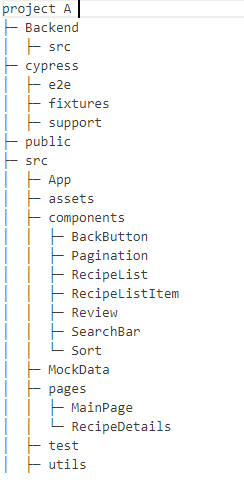
\includegraphics[width=0.30\textwidth]{Figures/A_Structure.png}\label{fig:A_stru}}
  \hfill
  \subfloat[B Structure.]{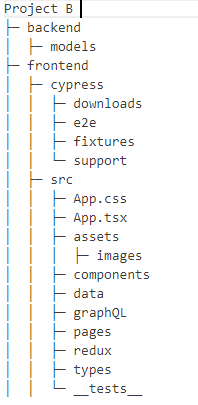
\includegraphics[width=0.29\textwidth]{Figures/B_Structure.png}\label{fig:B_Stru}}
  \hfill
  \subfloat[C Structure.]{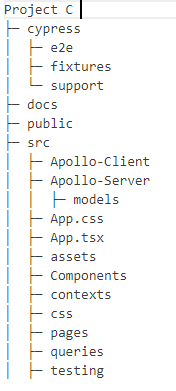
\includegraphics[width=0.27\textwidth]{Figures/C_Structure.png}\label{fig:C_Stru}}
  
\label{fig:Test_Structures}
\end{figure} \hfill 



\subsubsection{Control Project}
The control project is an open source project found on GitHub called "Hydra\footnote{https://github.com/hydralauncher/hydra}", written in TypeScript. Hydra is, as of 16.06.2024, a game launcher with 44 contributors and 1030 commits. This project serves as a control to validate the selection techniques against a larger and more complex codebase than typical student projects. By applying the selection methods to Hydra, the objective is to determine if these techniques are sufficiently accurate and inclusive when used on a substantially larger project. \\

By testing these selection techniques on both student projects and a substantially larger open-source project, the goal is to evaluate their effectiveness in different contexts. This approach aims to ensure that they provide meaningful insights and improvements to the Peer Code Review practice. \\

\noindent \textbf{Project Structure} \\
\noindent To get an overview of how the control project looks, Figure \ref{fig:Control_Structure} shows a simplified view of the project structure. Some folders are not included to make the figure readable. Only folders and sub-folders are shown. The project contained 172 files with the extensions; \textit{.ts, .js, .tsx, .jsx, .css, .html or .json}.


\begin{figure}[H]
    \centering
    \caption{Control Project structure} 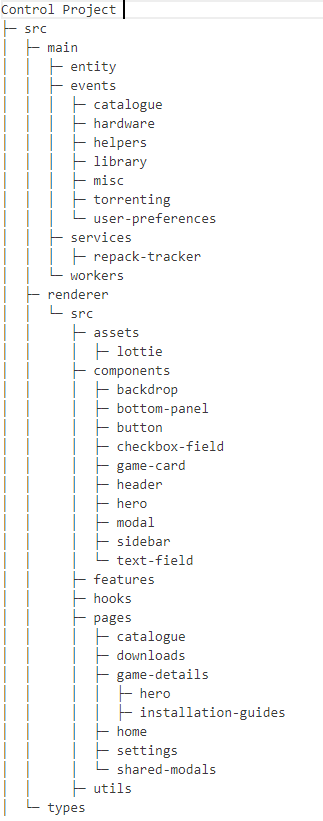
\includegraphics[width=0.3\textwidth]{Figures/Control_Structure.png}
    \label{fig:Control_Structure}
\end{figure}



\subsection{Evaluation Method}
To assess the efficiency of the various selection techniques, a controlled experiment was carried out on all the test projects, as well as the control project. Each technique was applied to the projects uniformly, which resulted in the selection of eight files by each technique for each project that, in total, resulted in 128 file selections. The files selected by each technique were then sorted into a priority list based on their metric scores. Specifically, Size Selection prioritized based on lines of code, Keyword Selection prioritized based on the occurrence of the specified keywords, Cyclomatic Complexity Selection prioritized based on the Cyclomatic Complexity score and Combination Selection prioritized based on the FTA score. During this process, the behavior of each selection technique was also observed to identify patterns or anomalies. \\

Before this, an \textit{Optimal Selection} list for each project was compiled by manually reviewing each file to determine the eight most important files for PCR. Prioritization was based on a holistic view of the project based on the logic, functionality, and complexity of the files. This meticulous process produced a benchmark list of optimal selections, which was used to assess the effectiveness and accuracy of each technique. Subsequently, comparisons were made between the files selected by each technique and the optimal selections. The consistency of each selection technique was also assessed by noting the frequency with which they identified the same files. If several selection techniques identified the same files, it suggested that these files were indeed more crucial, regardless of their inclusion in the Optimal Selection list.

%BESKRIVE DATAEN LITT GRUNDIGERE. HVA JEG HAR TESTET DET PÅ. GI LITT FAKTA. SYSTEMATISK EVALUERING MOT OPTIMAL SELECTIONS. MEN OGSÅ KJØRT EKSPERIMENTER FOR Å SE OPPFØRSELEN TIL TEKNIKKENE.